\documentclass[10pt,brazil]{article}

\usepackage{babel}
\usepackage{graphicx}
\usepackage[utf8]{inputenc}
\usepackage{ulem}


\title{O Incrível Manual de \sout{LaTeX} Yarco Super-Híper}

\author{André Mesquita Pereira \and Henrique Gemignani Passos Lima \and Renan Teruo Carneiro}

\begin{document}

\selectlanguage{brazil}

\maketitle

\begin{abstract}

Este artigo apresenta, de forma didática e divertida, o funcionamento
do \sout{\LaTeX} Yarco, que é um \sout{formatador de textos científico} jogo criado por \sout{Leslie
Lamport} nós a partir do programa \sout{\TeX} EP3 criado \sout{pelo} pelos \sout{pai dos algoritmos} POGgers,
\sout{Donald Knuth} nós, no início da década de \sout{1970} 2010.\footnote{Esse trecho não foi, sob hipótese alguma,
retirado do exemplo em sala de aula.}

\end{abstract}

\section{Introdução}

Como diz o enunciado do EP:

\begin{quote}
Estamos nos primeiros anos do século XX. O imponente transatlân- tico RMS Positronic deixa a Europa rumo ao Novo Mundo.
 Tudo corria bem em sua viagem, até que o navio esbarrou em um iceberg (sim, clichê básico de tragédias marítimas).
 Todavia, para a felicidade dos passageiros, o navio seguia rigorosamente os protocolos de segurança e havia coletes
 salva-vidas para todos. Outra sorte é que era verão na época do naufrágio, dessa forma tampouco as vítimas tiveram
 problemas com hipotermia.

Felizmente para os passageiros, quis o destino que próximo ao naufrágio passasse o modesto navio cargueiro Asimov. O cargueiro, que contava com dois botes, prontamente colocou-os para o resgate dos passageiros em alto-mar.
\end{quote}

O objetivo do jogo é controlar ambos os botes para resgatar o maior número possivel de passageiros do
recém-falecido RMS Positronic.

E Yarco ainda é um nome misterioso. Tentamos inventar um backronym para ele, mas sem muito sucesso até o momento.

\section{Instalando o Yarco}

Com um pouco de sorte (Leia-se: O responsável pelo autoconf terminou sua parte a tempo), o pacote incluirá um configure
funcional. Nesse caso, basta rodar o configure, rodar o make, e ser uma pessoa feliz. Caso isso não seja uma verdade,
o configure ainda não está pronto, e nesse caso a gente culpa novamente o Haruki. Aí um make sozinho se encarrega de
gerar o jogo. Caso você ainda não tenha rodado o configure. Caso tenha rodado, meus pêsames.

Para remover o jogo, basta um make clean. Para remover todos os arquivos gerados, um make realclean resolve. E caso nunca
mais queira ver esse projeto, make nuke é a opção preferencial.

\section{O Jogo}

Agora que todos nós perdemos, expliquemos como funciona o Yarco. Cada jogador controla um bote, com o objetivo de resgatar
or pobres passageiros do RMS Positron. Esse é um jogo estilo arcade, ou seja, dura até todos jogadores morrerem.

Para que você possa se situar, apresentaremos agora os elementos do jogo.

\subsection{O bote}

\begin{figure}
\begin{center}
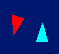
\includegraphics{boats}
\label{img:boat}
\caption{Os nossos queridos botes}
\end{center}
\end{figure}

Como você pode ver ver, na Figura \ref{img:boat}, os botes são triângulos simpáticos que você pode controlar. Eles são
capazes de remar para frente, para trás, de ancorar e de virar para os lados. Ele pode resgatar passageiros, mas lembre-
se de que eles não são coração de mãe, uma hora eles ficam cheios. Para desembarcar os passageiros resgatados no Asimov,
basta ancorar perto dele. Os passageiros lentamente subirão a bordo do Asimov e ficarão felizes ao ver que as pessoas mais
irritantes ainda não foram resgatadas.

\subsubsection{Os controles}

Todos os controles aqui descritos serão, respectivamente, para o primeiro e para o segundo jogador. Note que são os
controles padrão e que podem ser alterados.

Acelerar para frente: W e seta para cima\\*
Acelerar para trás: S e seta para baixo\\*
Virar no sentido horário: D e seta para a direita\\*
Virar no sentido anti-horário: A e seta para a esquerda\\*
Ancorar: Q e 0 no teclado numérico\\

\subsection{Os passageiros}

\begin{figure}
\begin{center}

\includegraphics{people}
\label{img:people}
\caption{Os nossos perdidos passageiros}
\end{center}
\end{figure}

Representados na Figura \ref{img:people}, os passageiros são bolinhas que ficam à deriva no mar, esperando serem resgatados.
Aparentemente, o RMS Positron era gigantesco, uma vez que nunca param de surgir mais passageiros.

\subsection{Os corais}

\begin{figure}
\begin{center}

\includegraphics{corals}
\label{img:corals}
\caption{Os nossos irritantes corais}
\end{center}
\end{figure}

Os corais podem ser vistos em seu habitat natural na Figura \ref{img:corals}. São quadrados de tamanhos e cores variados.
Eles são mortais, esbarrar em um deles significa um bote a menos na missão. E eles são capazes de geração espontânea,
então cuidado!

\subsection{O Asimov}

\begin{figure}
\begin{center}

\includegraphics{ship}
\label{img:ship}
\caption{O nosso importantíssimo Asimov}
\end{center}
\end{figure}

O grande retângulo cinza que você vê na Figura \ref{img:ship} é o Asimov. Ele fica paradão, tranquilo no meio da tela.
Para que passageiros sejam de fato resgatados, você deve ancorar pero dele, então nunca se esqueça de sua posição.

\section{Configurando o Yarco}

Você deve ter notado um arquivo chamado config.ini. Lá você pode editar o funcionamento do programa à vontade. Note que
a parte de controles envolve números, que correspondem às teclas pressionadas. Se o Makefile colaborar, deve estar dispo-
nível uma ferramenta que lhe dirá quais são os números associados a cada tecla. As configurações devem ser suficientemente
claras, então fica como exercício ao leitor descobrir o que cada uma faz.

Ou isso ou haverá um arquivo a parte explicando.

\section{Conclusão}

Pode-se dizer que foi  um projeto interesante, especialmente dado que o grupo simplesmente decidiu fazer tudo
em uma semana, devido a provas e a completa ausência de processamento multithreading na equipe. O resultado final
 é um tanto abaixo do esperado, mas pelo menos é jogável. Não existem testes, porque ninguém lembrou de fazer.
 Não há uma tela de início. E nem tem o Konami code! Mas, algo está feito. Pelo menos, espero eu, fica a lição de
não empurrar tanto um projeto com a barriga.

...E de não querer projetos próximos às datas de beta de StarCraft II e da copa.

\end{document}
